The finite difference scheme considered was the one used by Holden and Raynaud \cite{holden2006convergence}:
\begin{align}
m &= u - D_{-}D_{+}u, \notag \\ 
m_t &= -D_{-}(mu) - mD(u),
\label{eq:discretized}
\end{align}
where the operators are defined as
\begin{align}
\label{eq:operators}
D_{+}u_{j}^{n} = \frac{u_{j}^{n}-u_{j-1}^{n}}{h},\quad
D_{-}u_{j}^{n} = \frac{u_{j+1}^{n}-u_{j}^{n}}{h},\quad
D = \frac{D_{+}+D_{-}}{2}.
\end{align}
The main disadvantage of this scheme is that one has to assume only positive values of $u$. However, it is debatable whether a negative $u$ makes sense or not.

Our finite difference scheme is based on a scheme presented by Morten Lien Dahlby\cite{dahlby2007geometric}, and is a slight modification of the scheme presented by Holden and Raynaud.

\begin{align}
m &= u - D_{-}D_{+}u, \notag \\ 
m_t &= -D_{-}(m(u \vee 0)) -D_{+}(m(u \wedge 0)) - mD(u), 
\label{eq:modscheme}
\end{align}
where $(u \vee 0) = \text{max}(u,0)$ and $(u \wedge 0) = \text{min}(u,0)$.

The original scheme by Holden and Raynaud used the $D_{-}$-operator, making it an upwind method. This would not work for antipeakons. Modifying the scheme to use  $D_{-}$ when $u > 0$ and $D_{+}$ when $ u < 0$ makes it applicable to waves traveling in either direction. This modifications also makes the scheme able to handle more initial conditions and genereally makes the method more stable. 

To find an appropriate time step, the Courant–Friedrichs–Lewy (CFL) condition was considered. The CFL condition is a necessary condition for stability in our finite difference scheme, and can be stated as
\begin{align*}
c\frac{\Delta t}{\Delta x} \leq 1,
\end{align*}
where $c$ is the velocity of the wave, $\Delta t$ is the length of the time step, and $\Delta x$ is the length of the spacial step. Rearranging this inequality gives an expression for $\Delta t$:
\begin{align*}
\Delta t \leq \frac{\Delta x}{c}
\end{align*}
An estimate for $c$ is found in the following way: Since we do not know how fast our waves move we use a simple heuristic. We translate all the area in the initial condition into a peakon (which always has the area $2c$) and thereby bound the the speed equal to the height of this peakon. A simple illustration can be found in Figures \ref{fig:area1} and \ref{fig:area2}. The same heuristic can also be used for antipeakons.


\begin{figure}
\begin{subfigure}[b]{0.49\textwidth}
                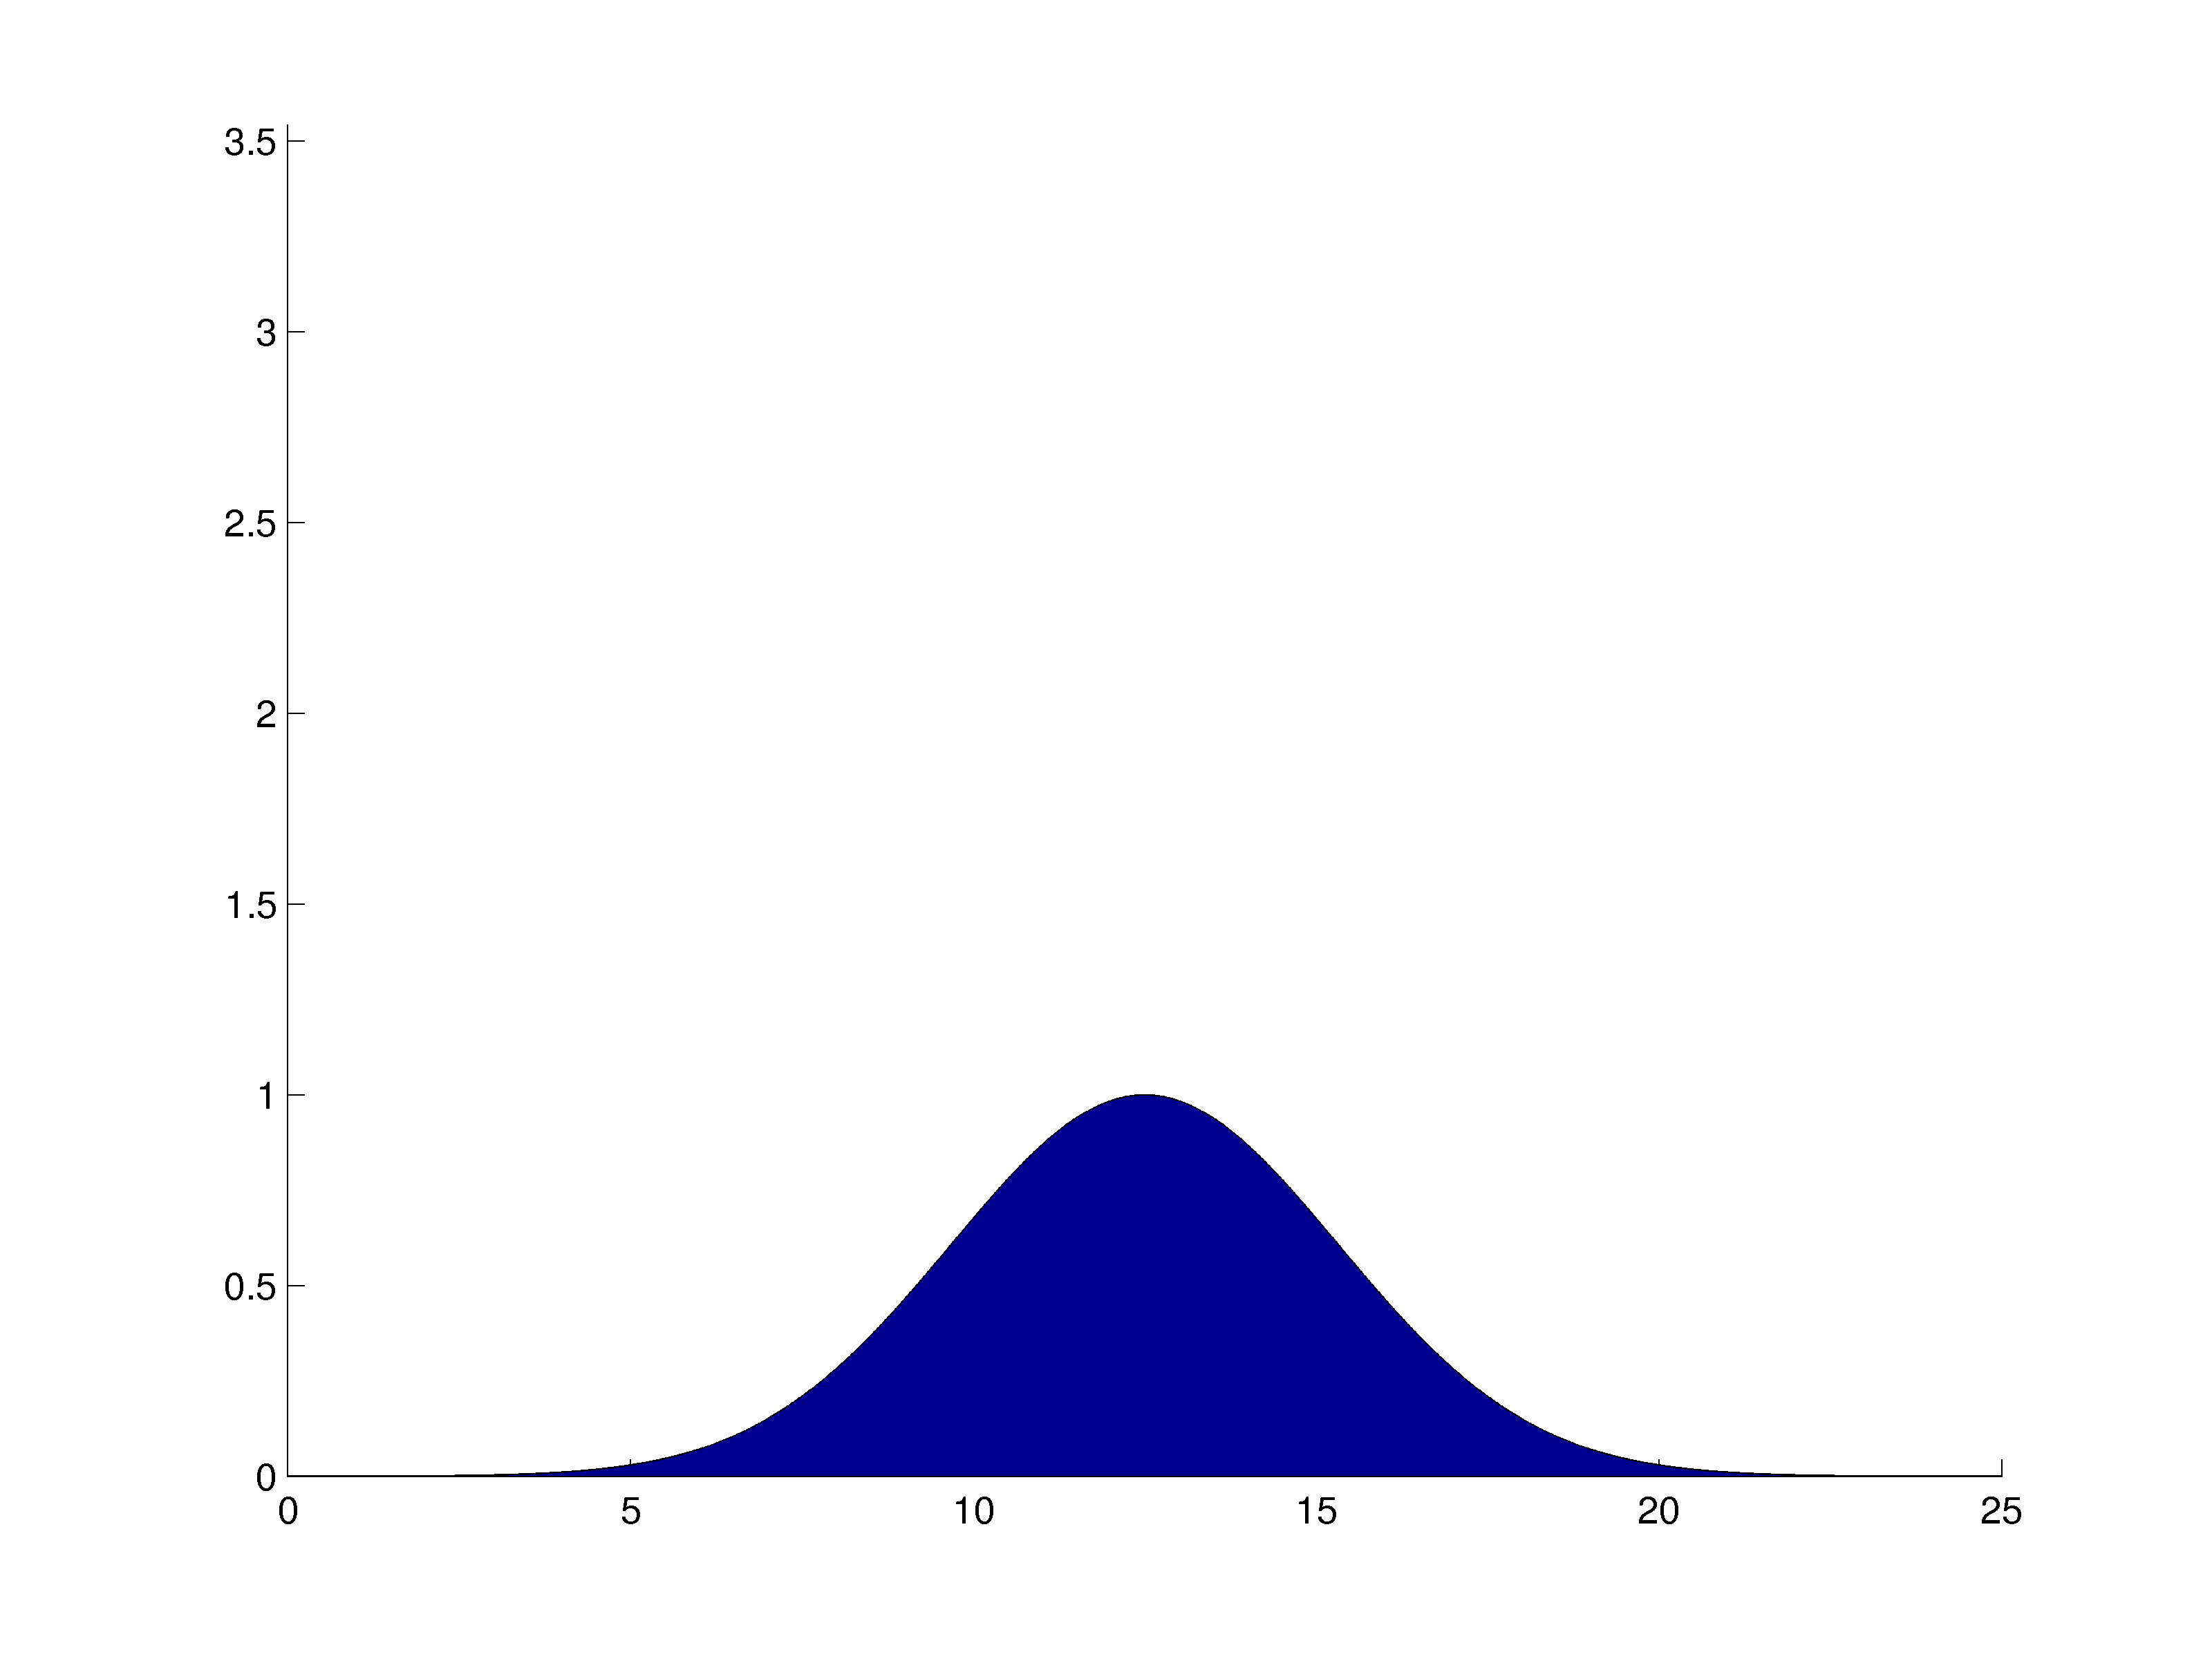
\includegraphics[width=\textwidth]{gfx/areainitial}
                \caption{Initial condition}
                \label{fig:area1}
\end{subfigure}
\begin{subfigure}[b]{0.49\textwidth}
                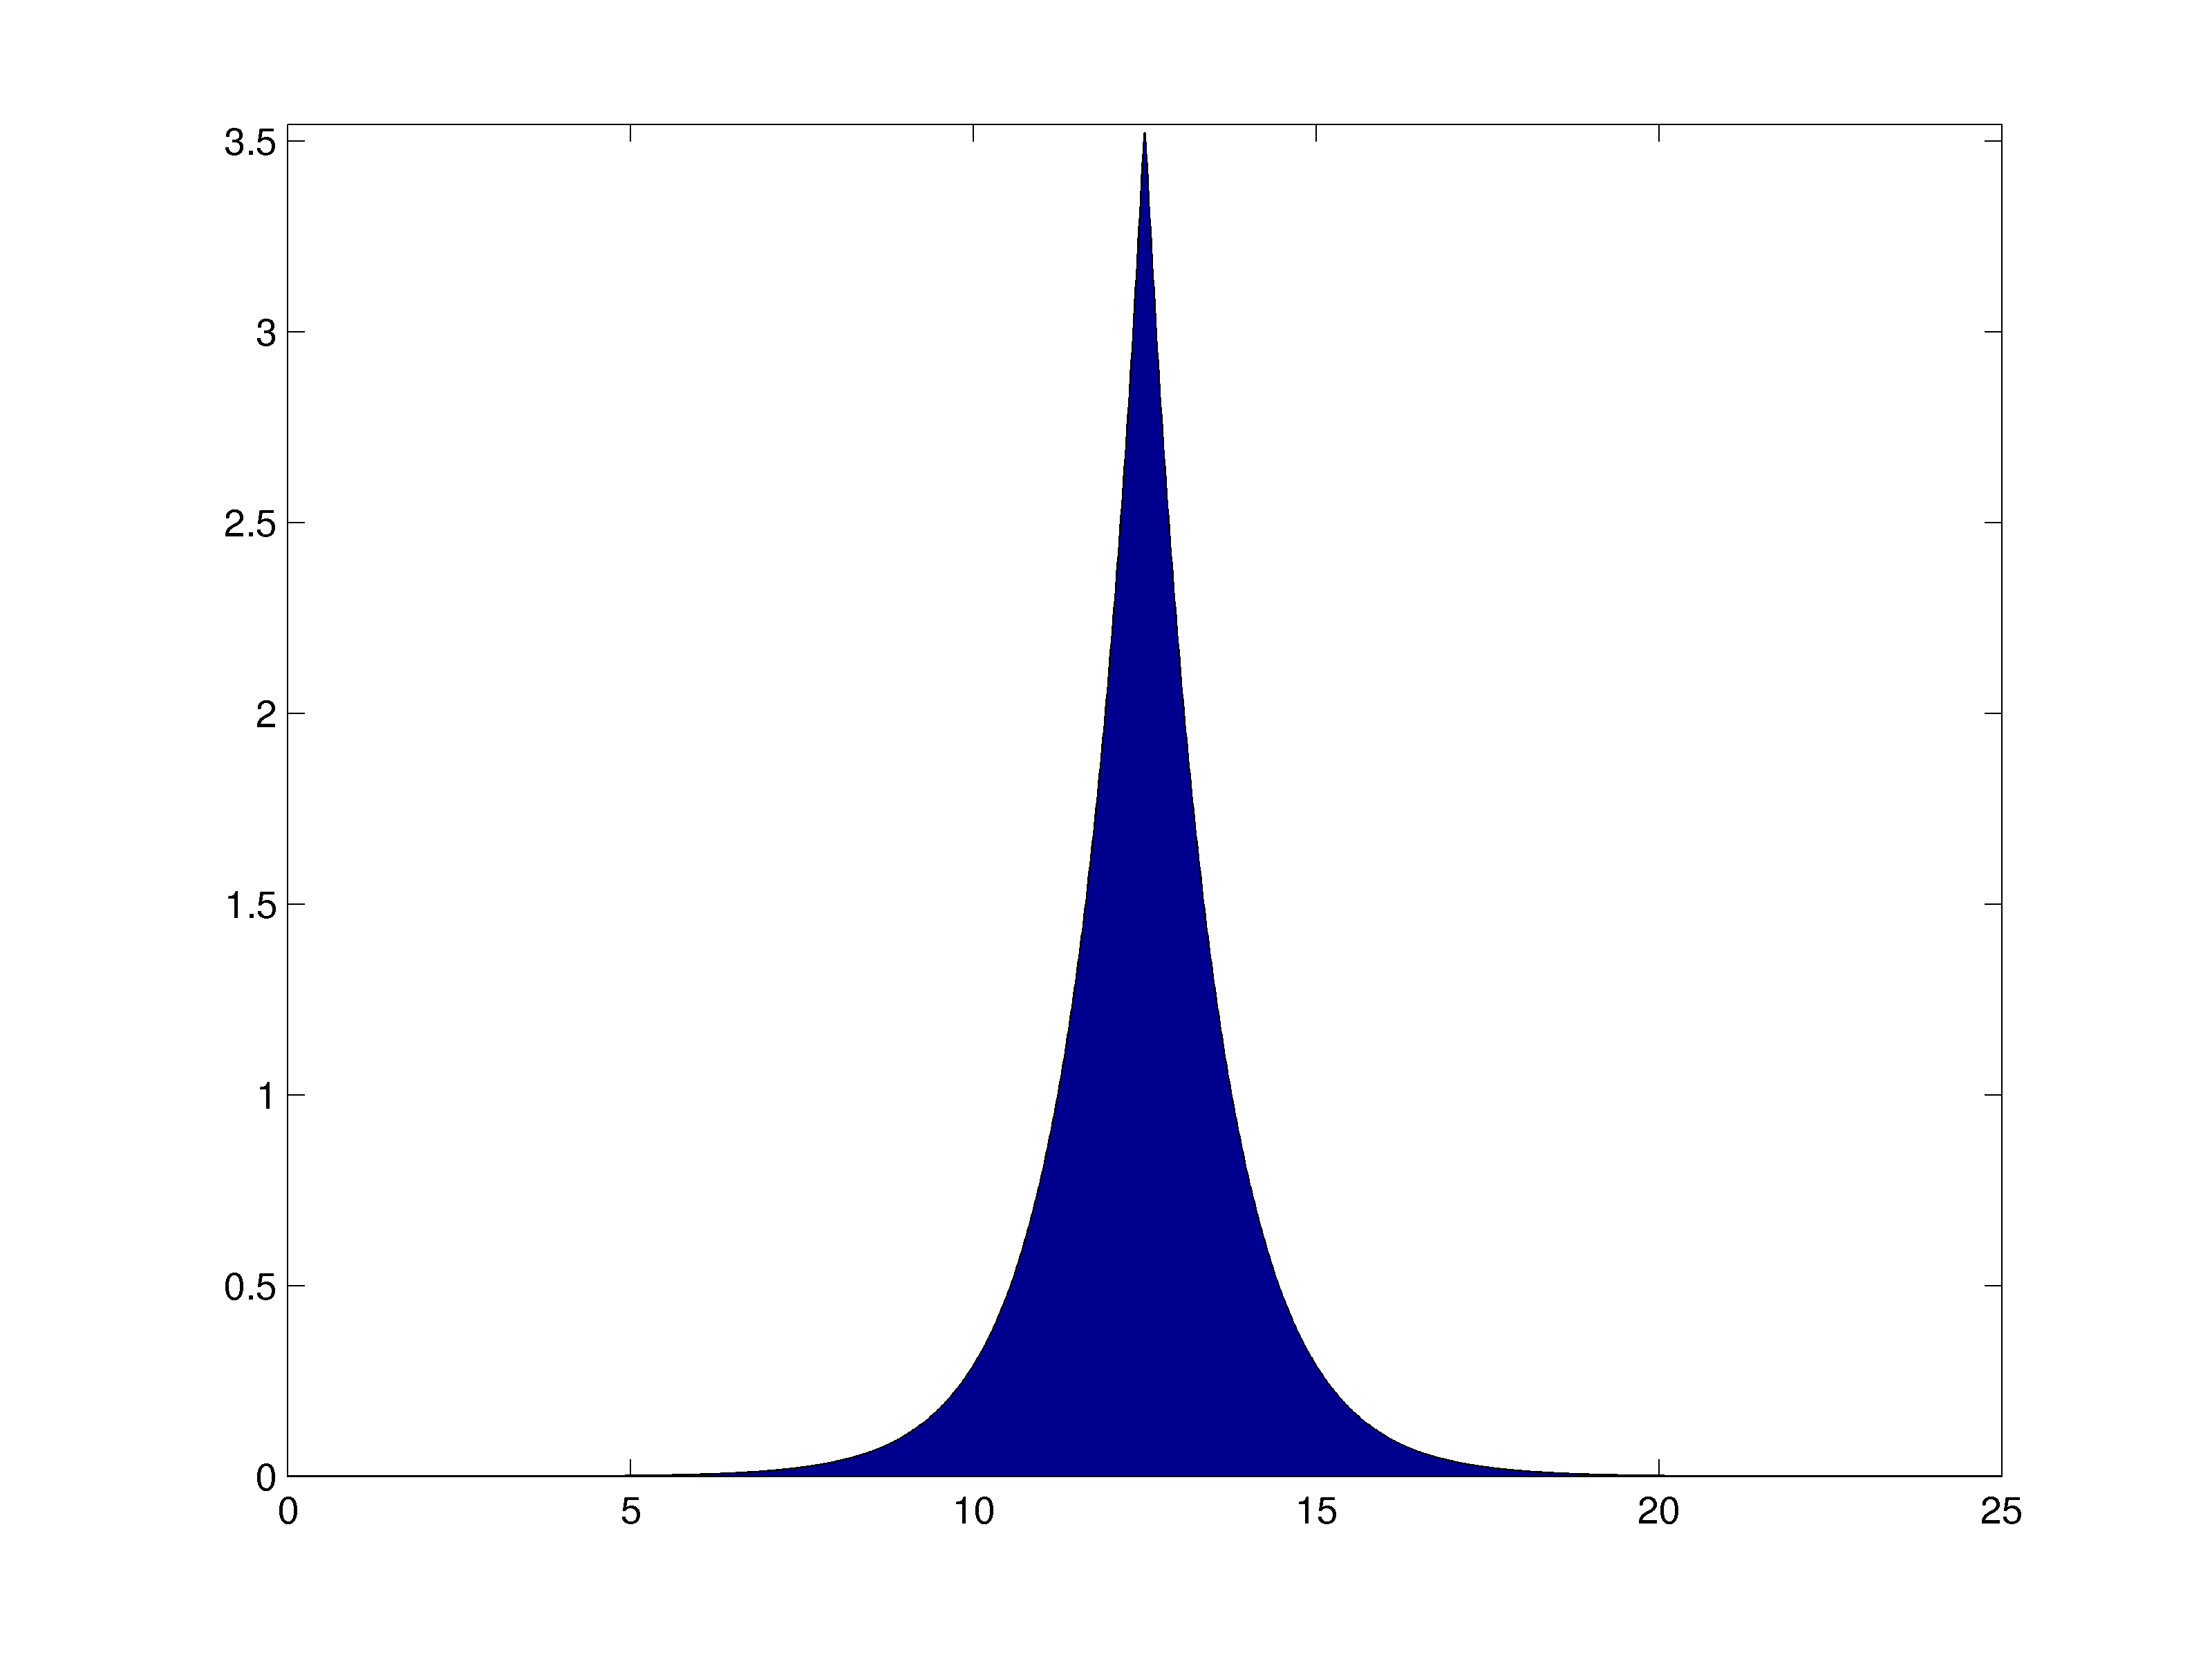
\includegraphics[width=\textwidth]{gfx/areapeakon}
                \caption{Peakon of same area}
                \label{fig:area2}
\end{subfigure}
\caption{Initial condition and peakon of same area, used to estimate $c$.}
\end{figure}


\subsection*{Correctness}

\begin{figure}[h]
        \centering
        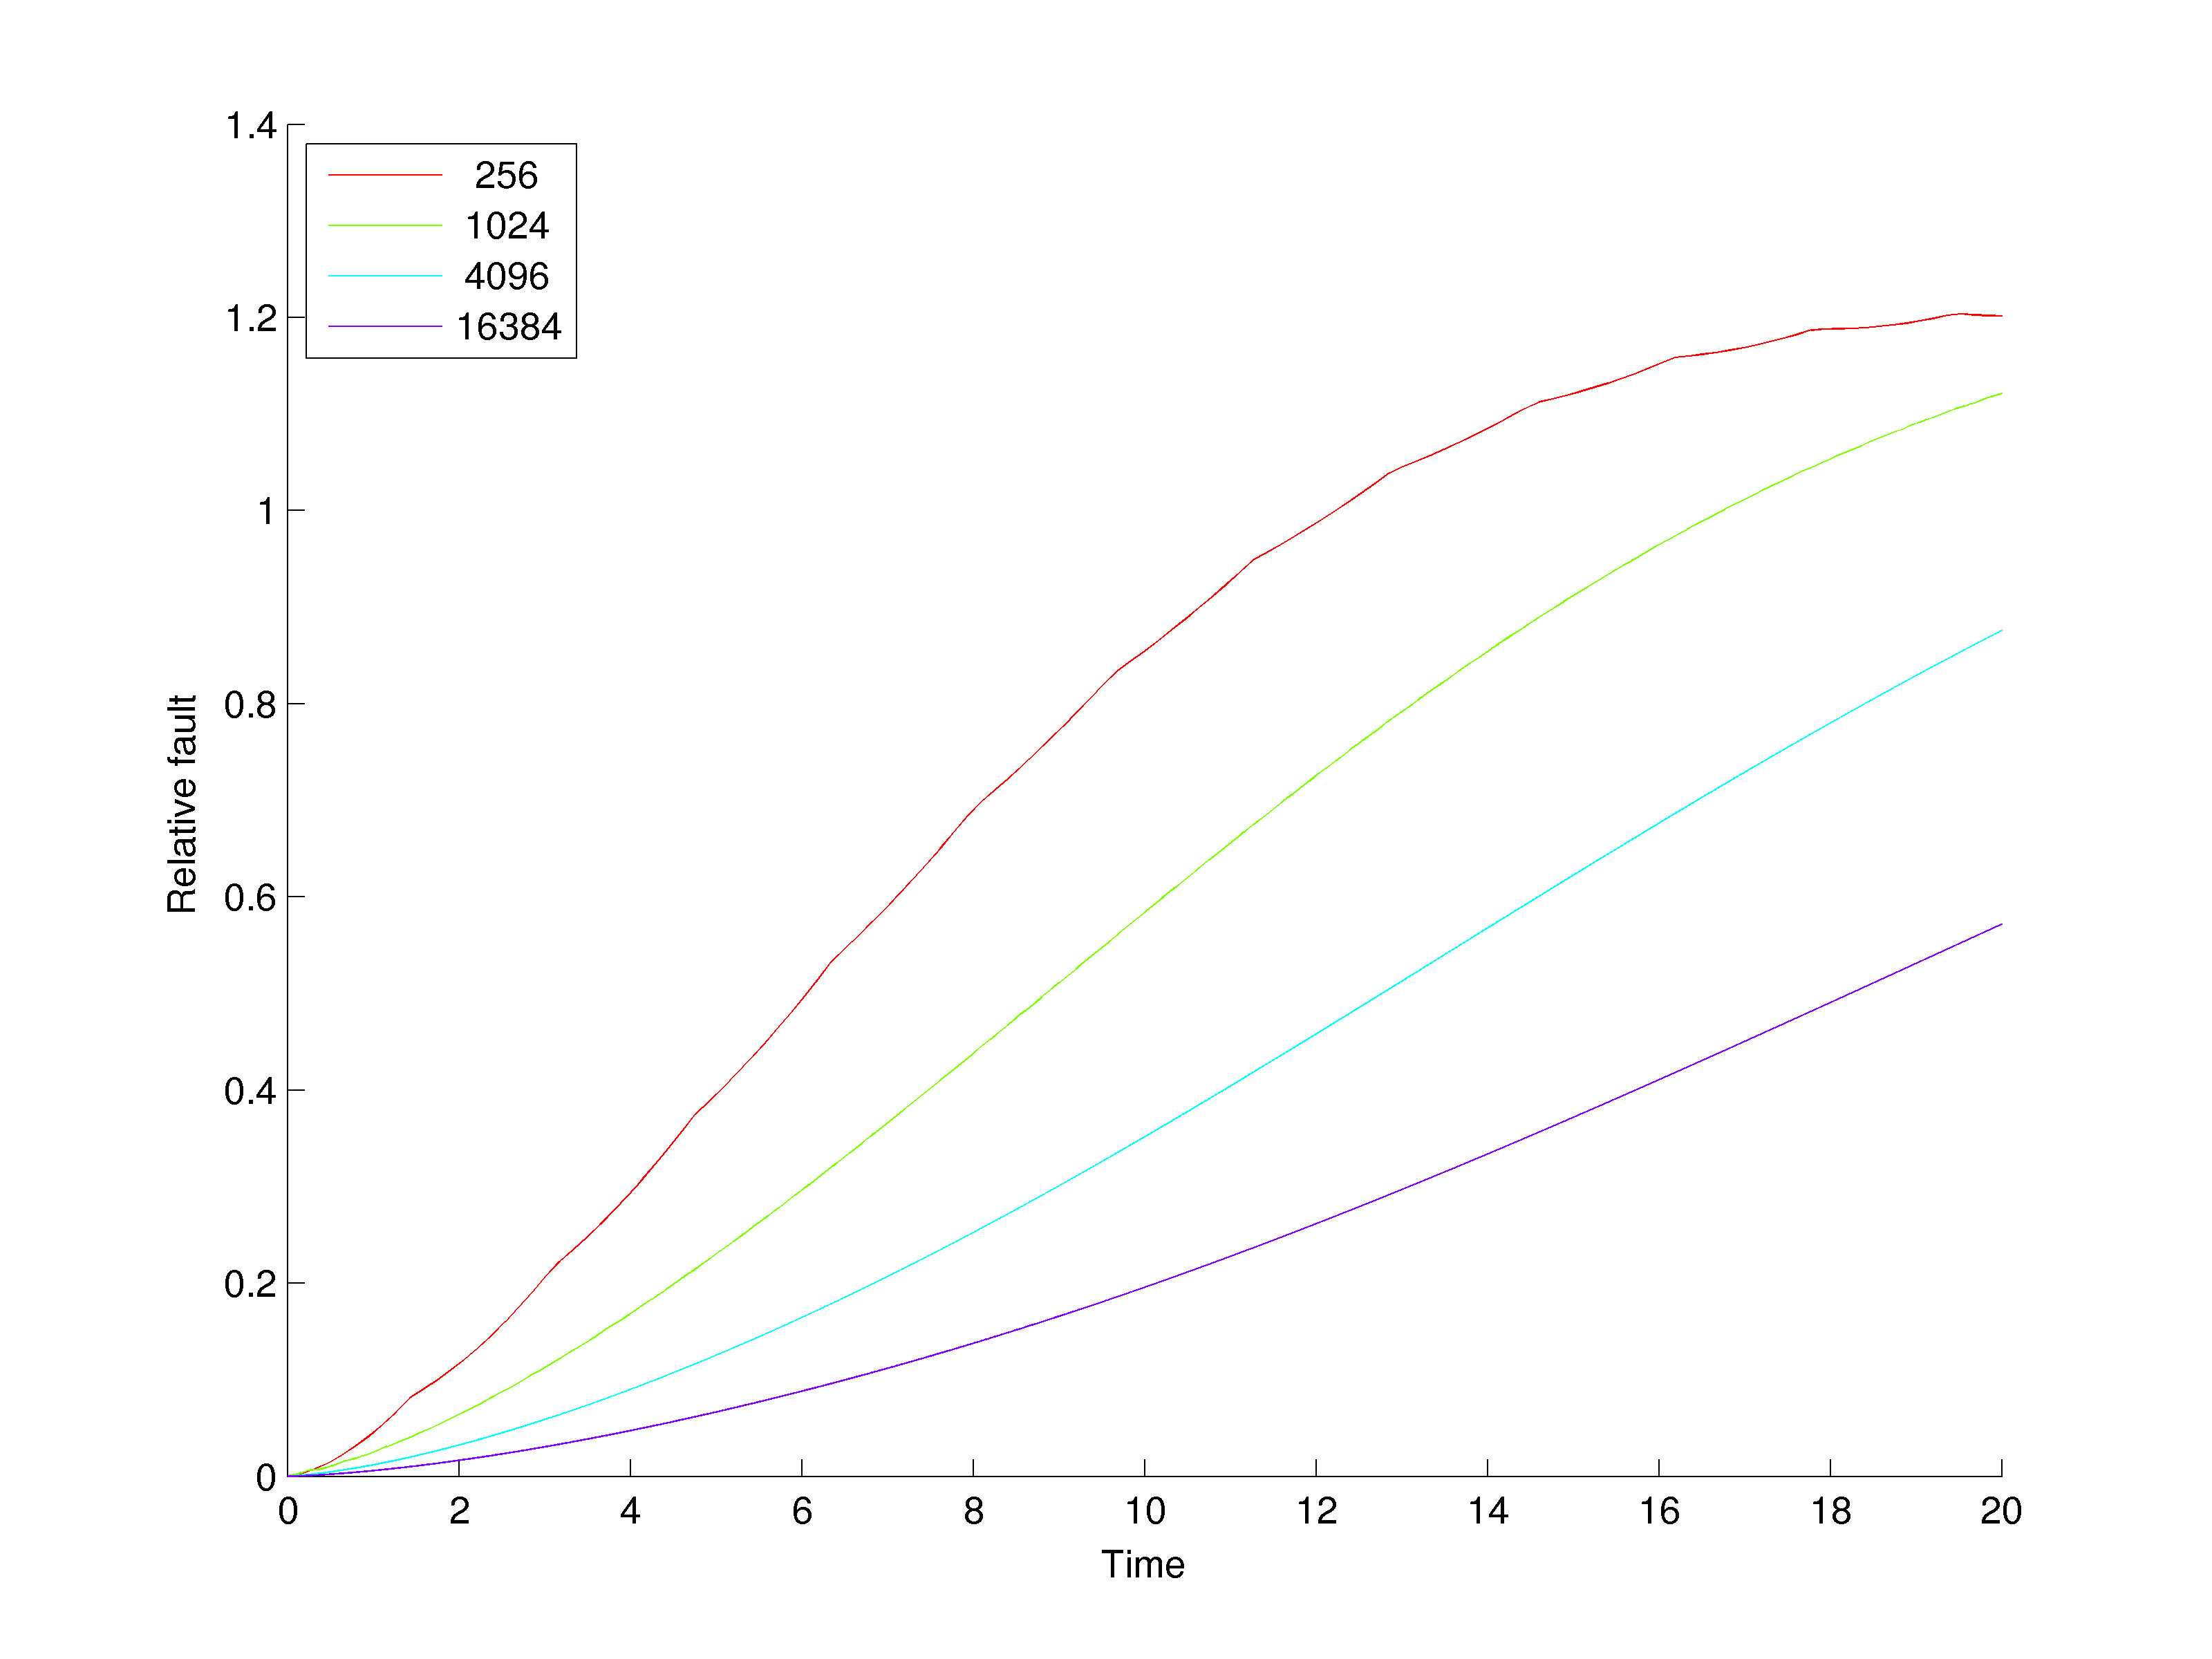
\includegraphics[width=0.8\textwidth]{gfx/erroroftime}
        \caption{Error plots for decreasing $h$, constant time and space interval. Initial condition: peakon centered in $x = 0$. End: analytical peakon lies at $x = 20$.}
        \label{fig:erroroftime}
\end{figure}
A preliminary conclusion based on the plot of errors for decreasing spacial stepsize $h$ (Figure \ref{fig:erroroftime}) shows that decreasing $h$ will improve the approximation. Figure \ref{fig:attimeT} shows that as the spacial stepsize $h$ decreases, our scheme becomes a good approximation of the solution. \\

\begin{figure}[h]
        \centering
        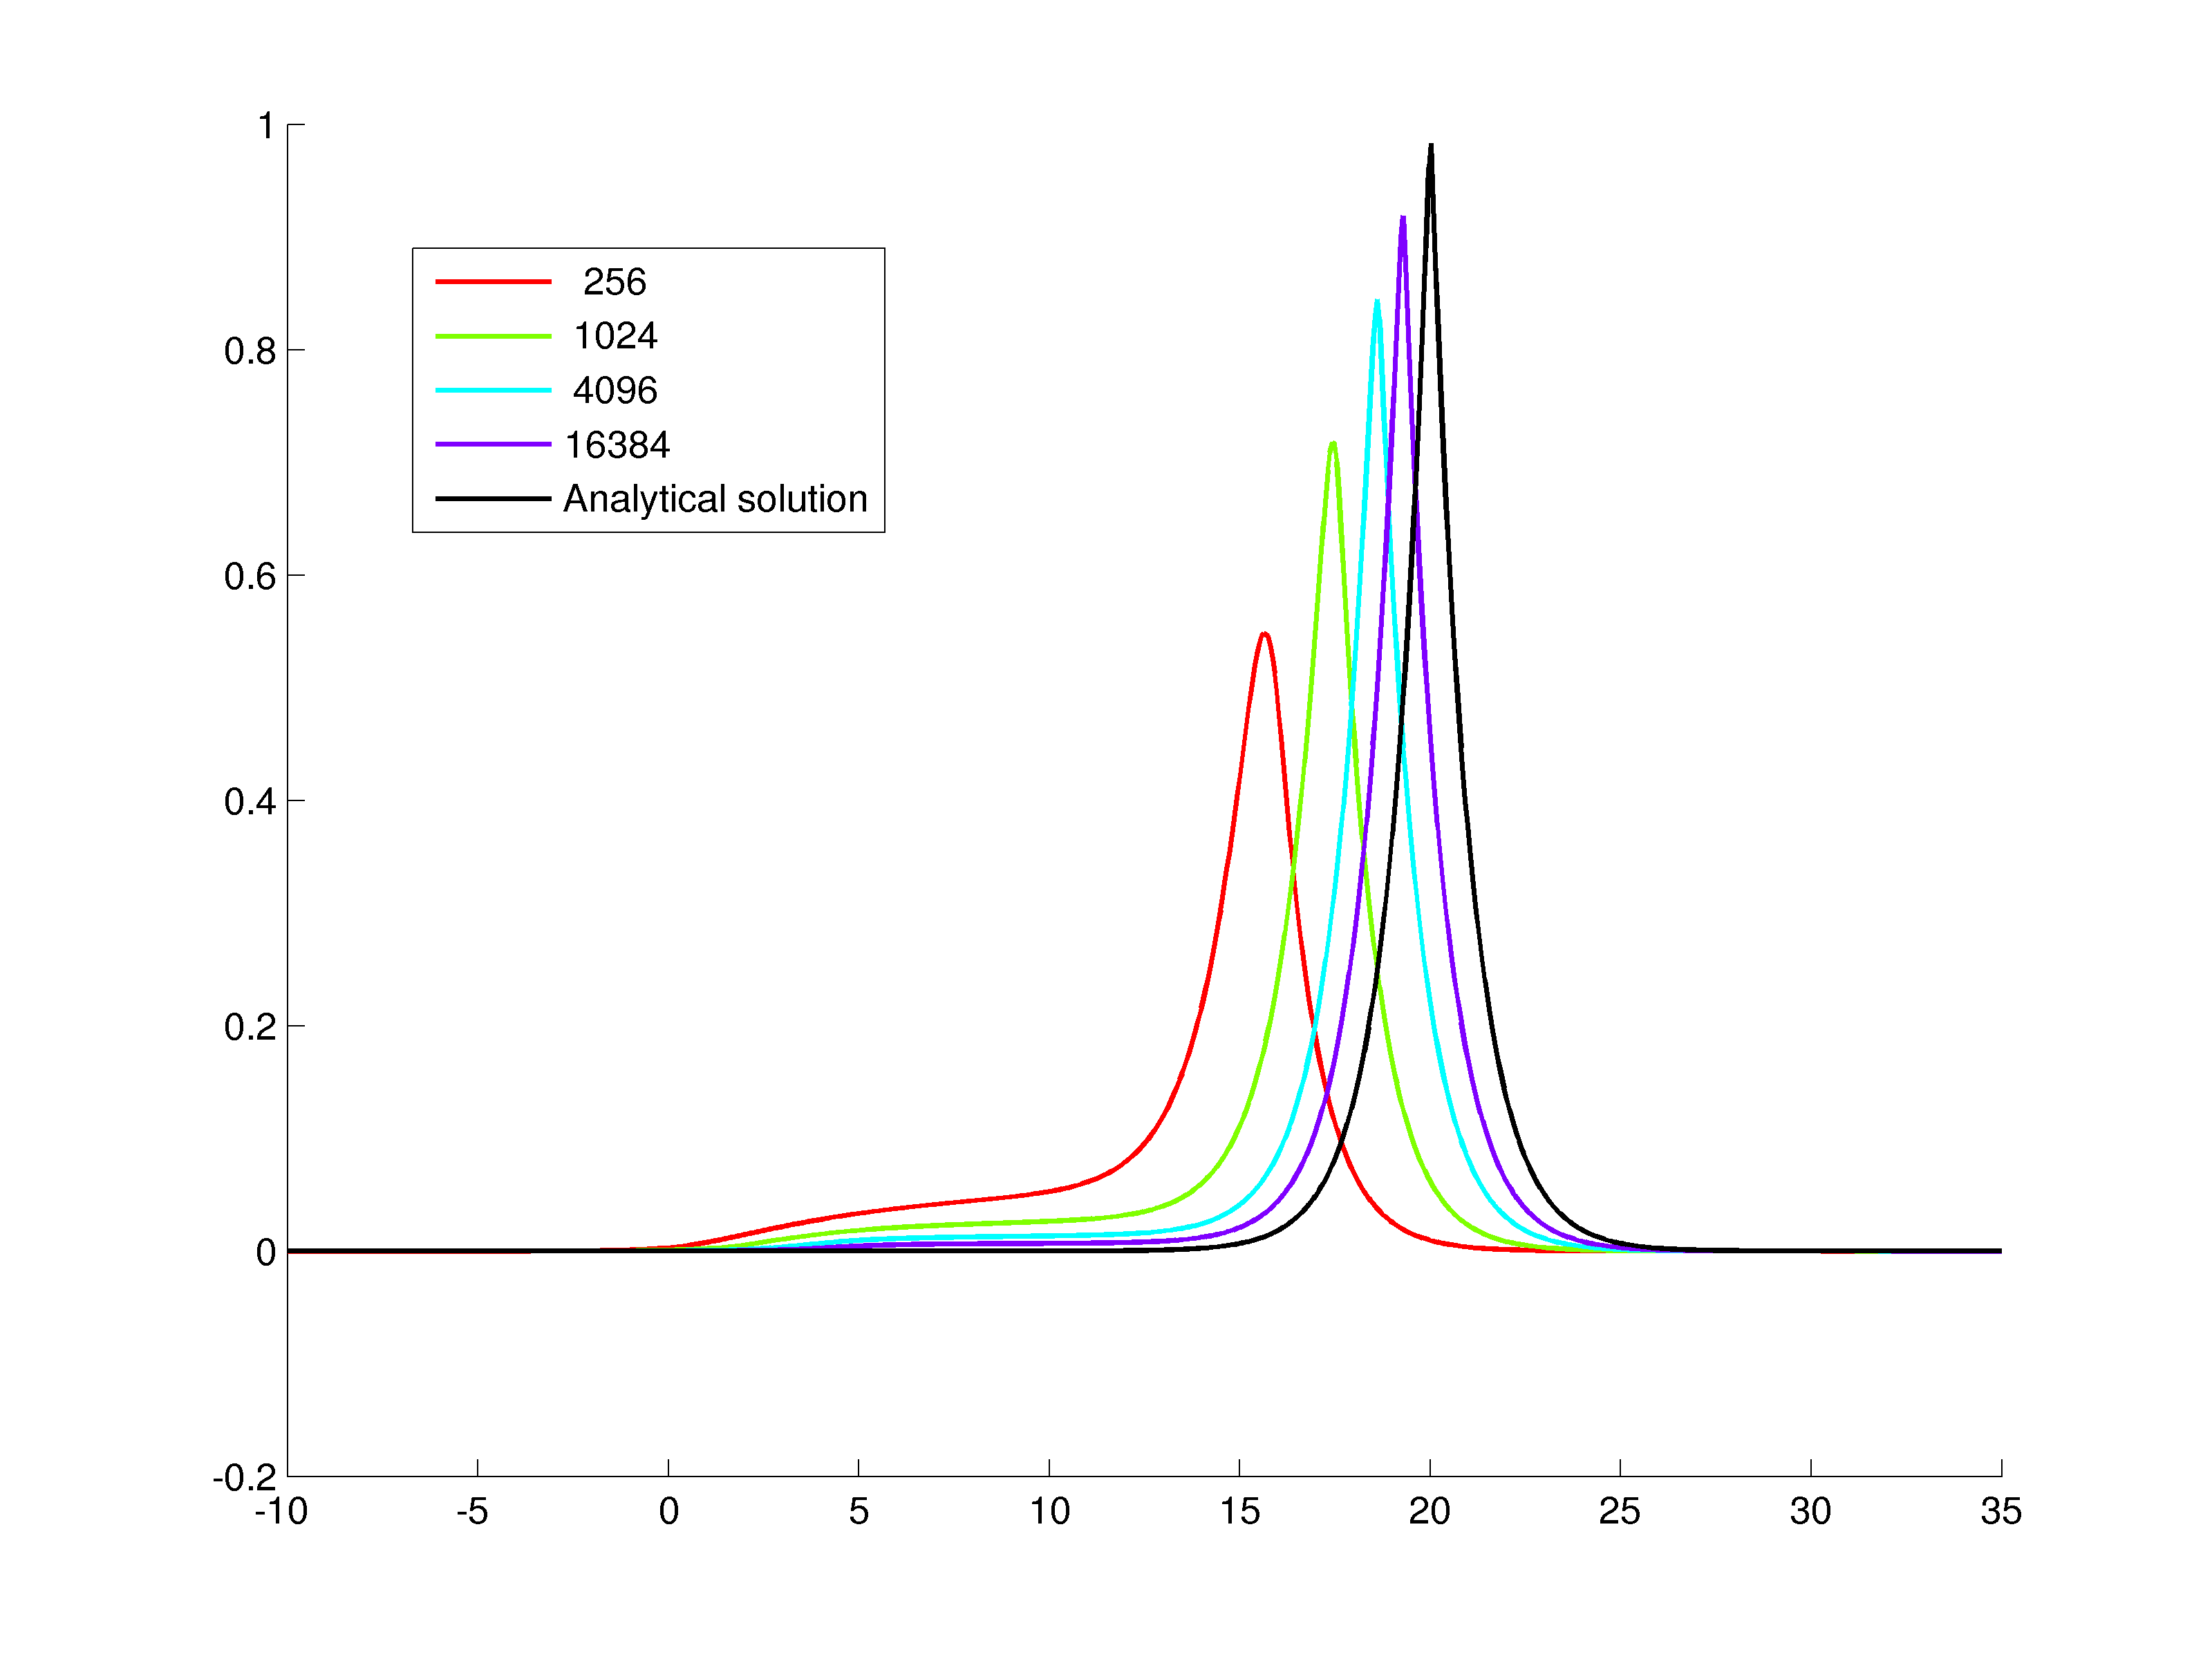
\includegraphics[width=0.8\textwidth]{gfx/attimeT}
        \caption{Plot of approximated solution together with analytical solution for decreasing spacial step $h$. Initial condition: peakon centered in $x = 0$.}
        \label{fig:attimeT}
\end{figure}

The Camassa-Holm equation has one critical property regarding convergence. Not only are the solutions discontinuous in the first derivative, the height is also equal to the speed. This means that any small error produced by a numerical method will amplify quickly. As the height of the peakon becomes lower it also becomes slower and thus quickly loses track of the analytical solution (at least for small grid sizes). If we make the endtime $T$ small enough, we are able to show linear convergence in space as shown in figure \ref{fig:loglog2}, with a constant time step. On the other hand, we are not able to show convergence in time (with a constant spatial step). See the loglog plot in figure \ref{fig:loglog2time}. It does not seem to converge to the peakon solution, but rather to a smooth wave with a bounded error. We have not managed to figure out why this happens. More about this phenomenon can be read in the section about semi-discretization. The fact that the solution gets worse with a small time step makes it important to pick the right time step. The bound on the time step presented earlier (from the CFL condition) works great. 
 

\begin{figure}[h]
        \centering
        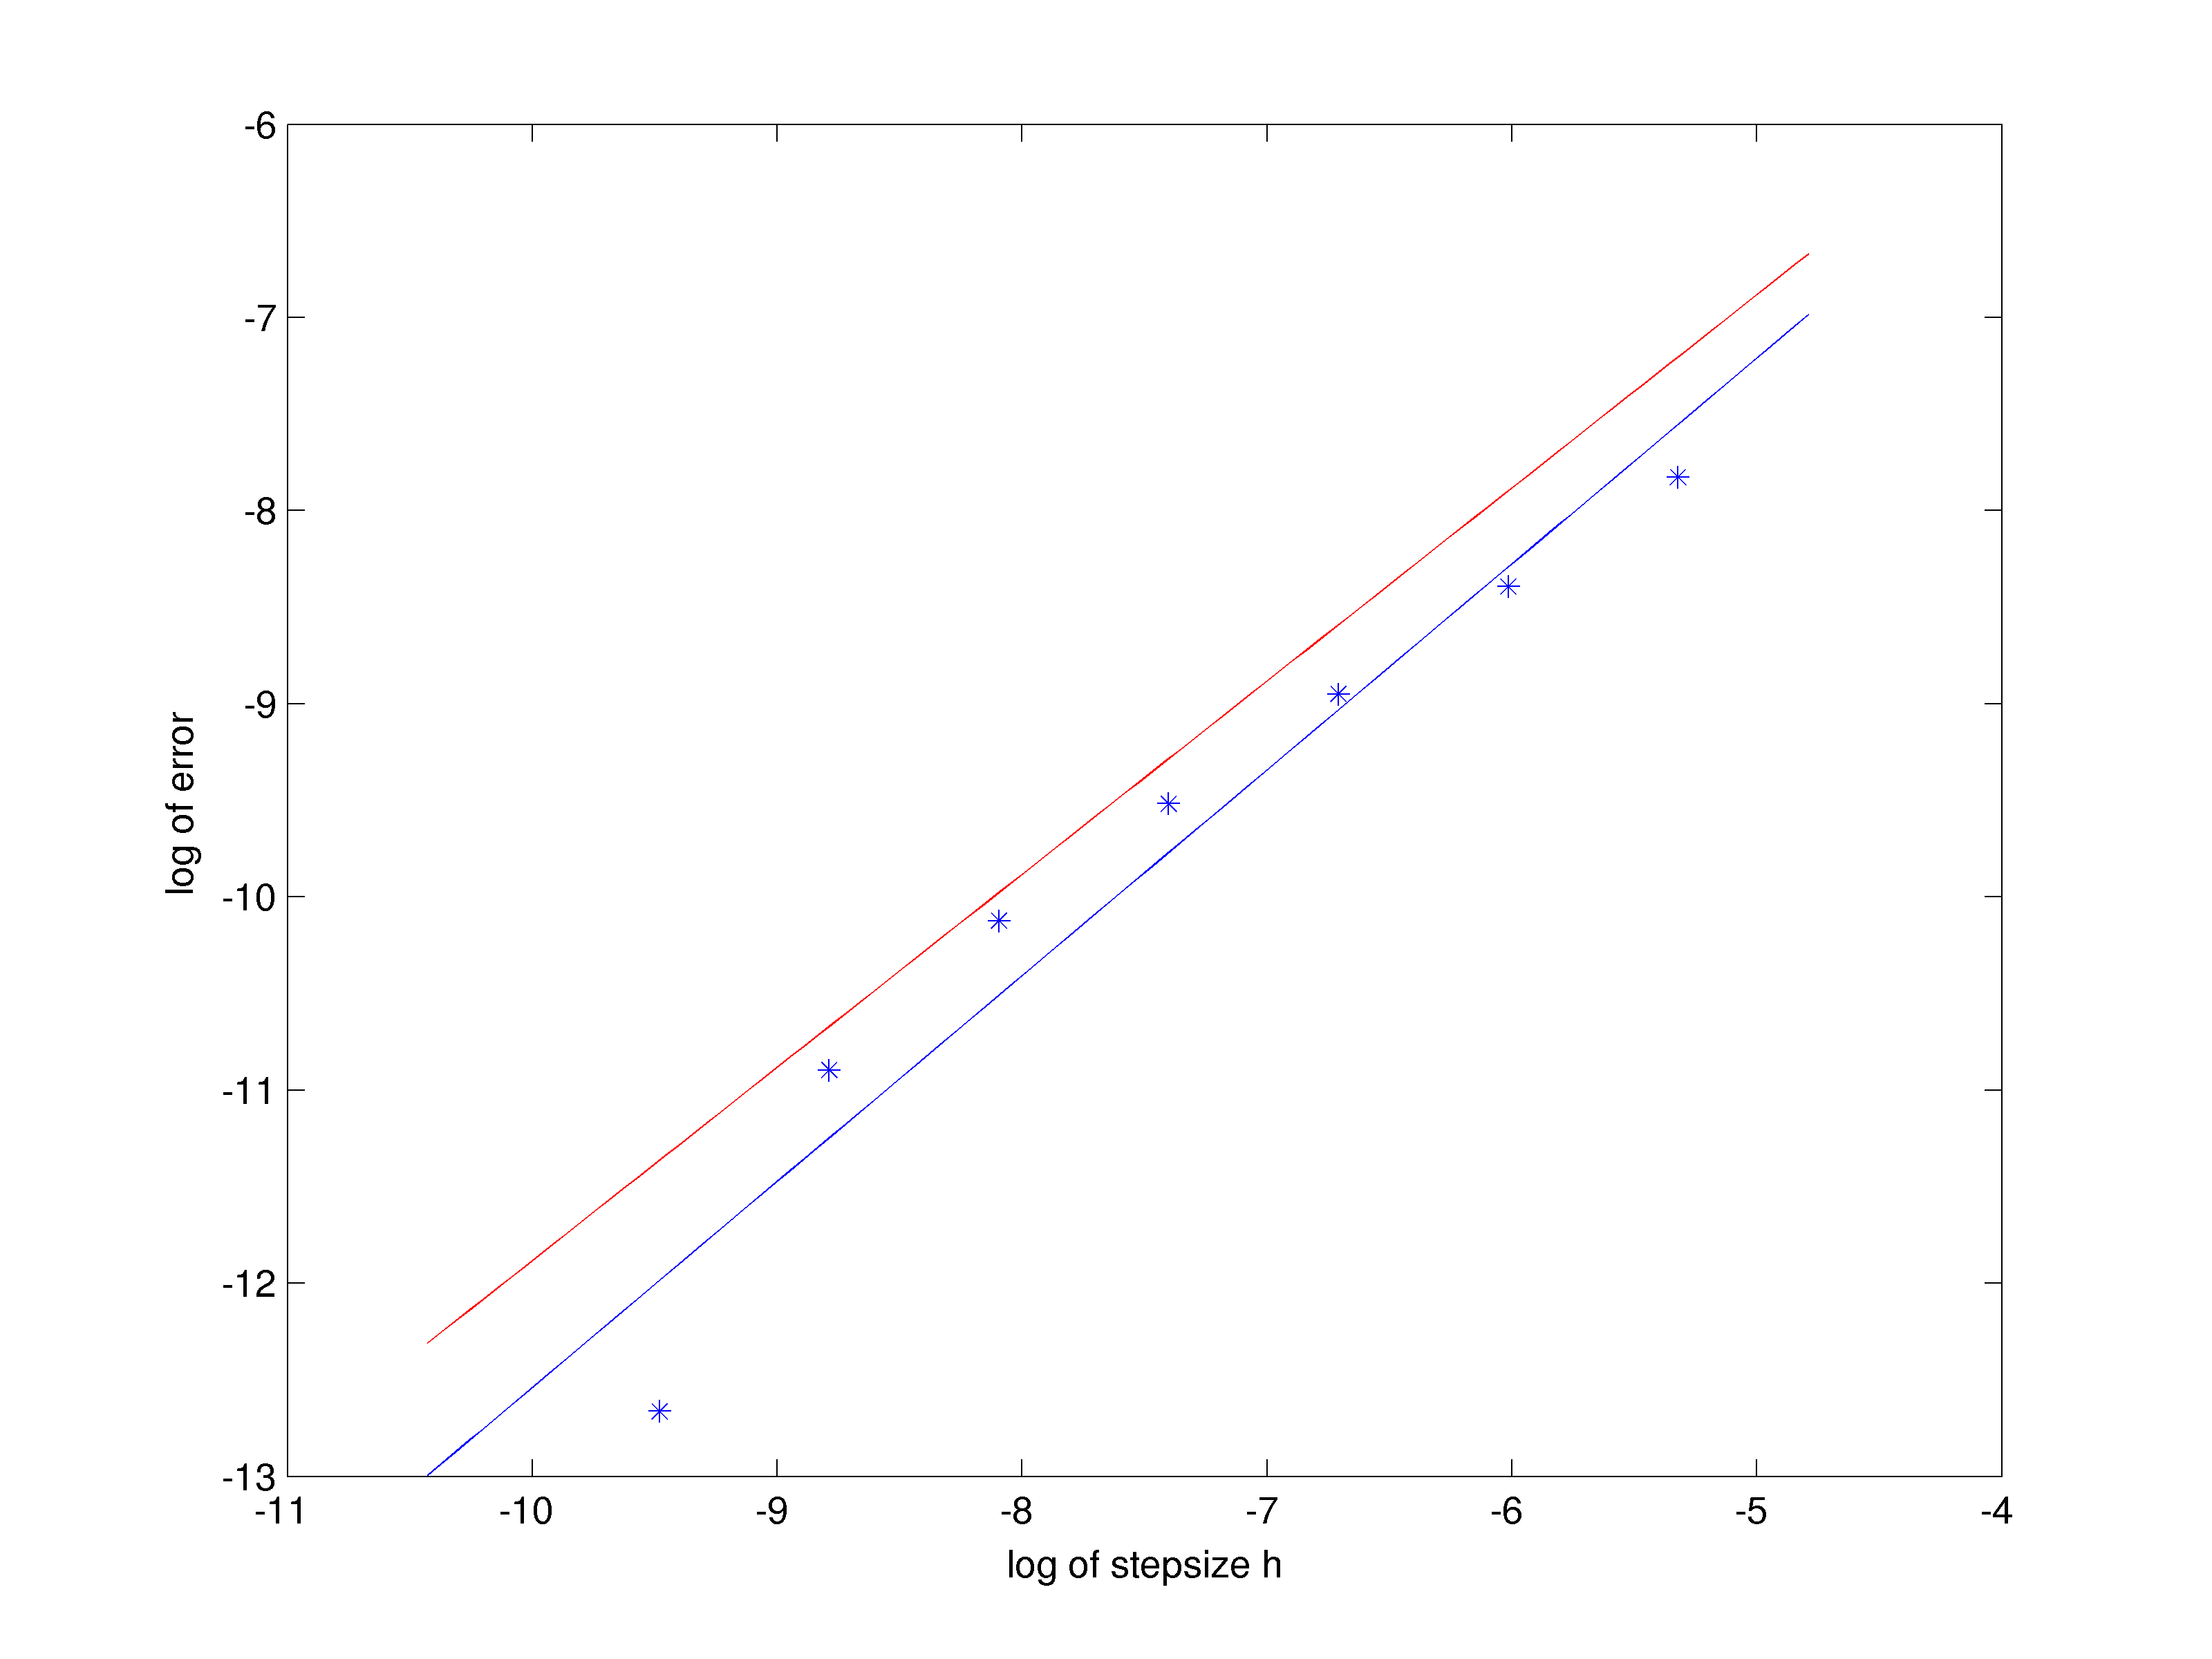
\includegraphics[width=0.8\textwidth]{gfx/loglog2}
        \caption{Loglog plot - rate of convergence in space. In this plot, the red reference line has a slope of 1, while the blue line found through numerical experiments has a slope of 1.07. $T = 0.01$, $t = 6.9 \cdot 10^{-5}$,$N = 2^{12}$ to $N = 2^{18}$.}
        \label{fig:loglog2}
\end{figure}

\begin{figure}[h]
        \centering
        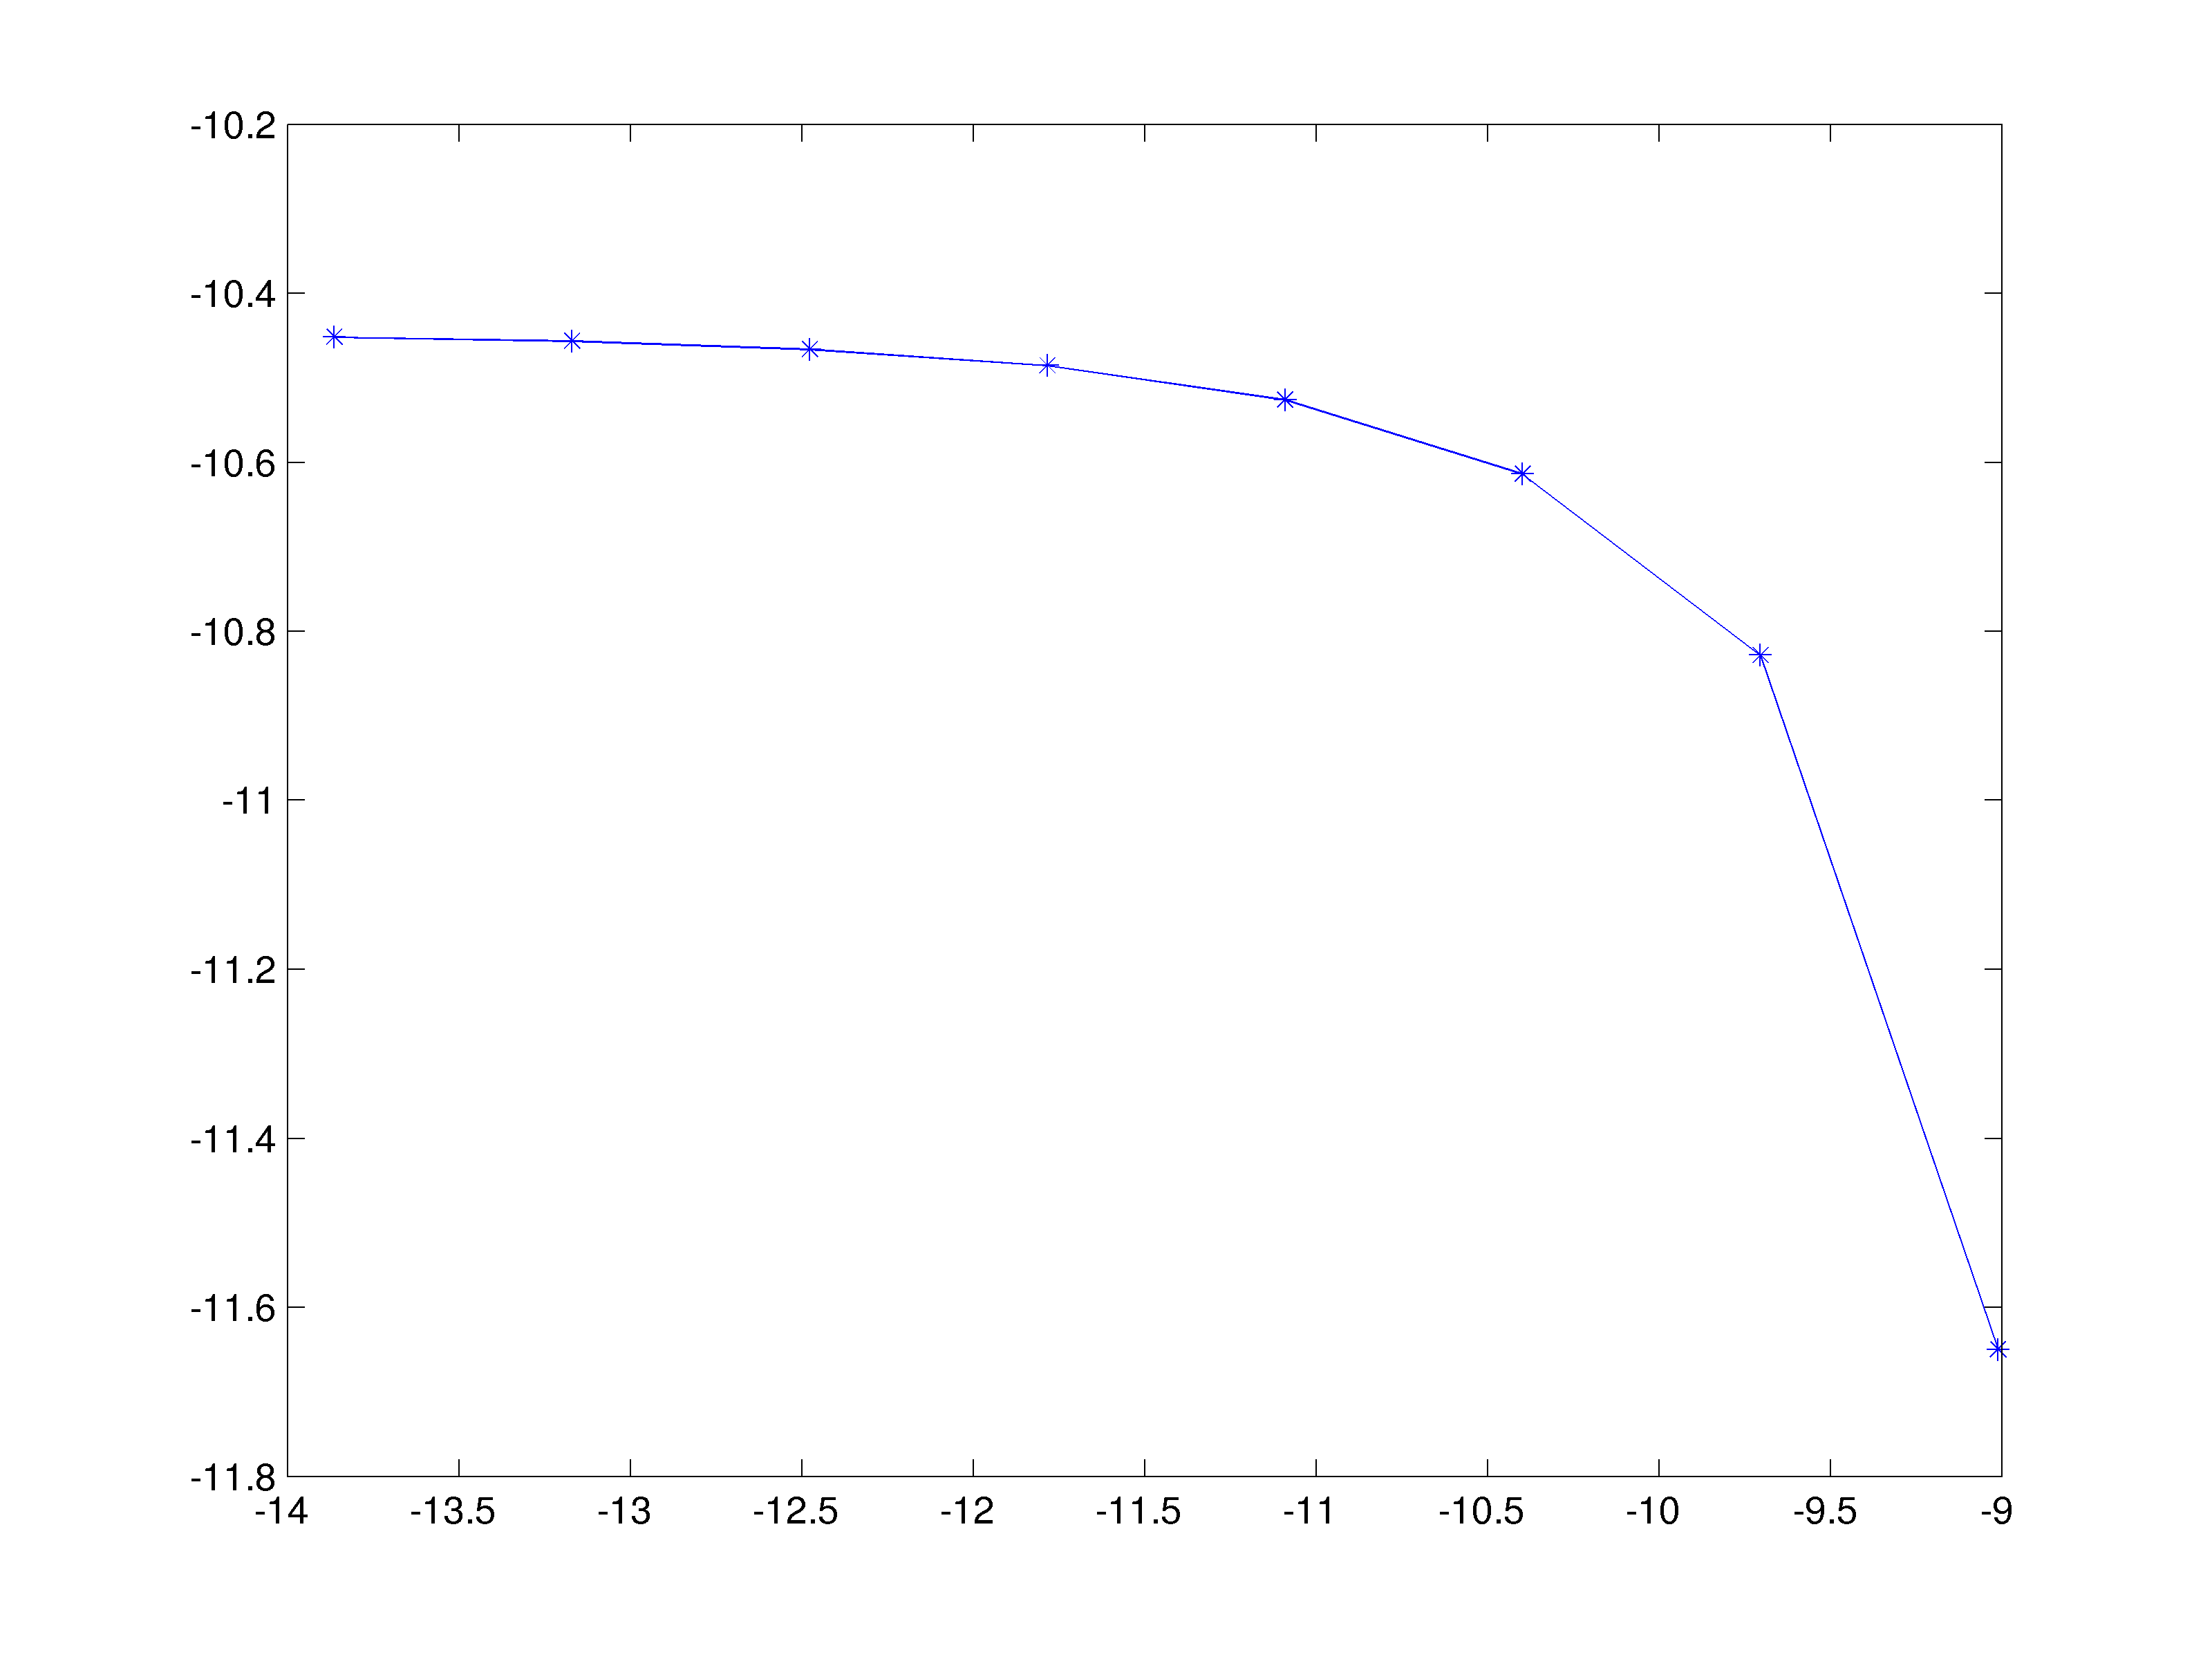
\includegraphics[width=0.8\textwidth]{gfx/loglog2time}
        \caption{Loglog plot - rate of convergence in time. The method does not converge in time. $T = 0.01$, $t = 2^{-13}$ to $ t = 2^{-20}$ and $N = 2^{17}$.}
        \label{fig:loglog2time}
\end{figure}



\subsection*{Semi-discretization}
Writing 
\begin{align*}
m_t = - D_- (m u) - m D u = f(m),
\end{align*}

one may obtain a system of ODEs which can be solved with standard numerical software, though each evaluation of $f$ requires a transformation from $m$ to $u$. Additionally, in the end one needs to transform the resulting matrix of $m$ values back to $u$. Testing a variety of MATLAB's built-in ODE solvers, including \emph{ode45}, \emph{ode15s} and \emph{ode113}, we surprisingly discovered that our explicit scheme based on Euler's method was far superior in every aspect to any other integrator available to us. 

The exact reason why is still unknown to us, though we suspect the discontinuous derivatives of the peakon solutions may cause problems for higher order schemes. This is at least consistent with the fact that the higher order schemes appear to smooth out the peaks of the solution.

Another interesting effect was observed when the time step of the explicit scheme was decreased (below the bounded value given by our CFL condition) with the spatial step fixed. Numerical experiments suggest that the solution offered by the explicit scheme converges towards the solution of the higher order time integrators as the time step goes towards zero. In other words, the increased error that results from too small time steps is somehow bounded by the higher-order schemes. We have not yet been able to discover the cause, and our only hypothesis is at best a farfetched and unlikely guess: perhaps our scheme somehow possesses innate damping, which is inaccurately underestimated by Euler's method in such a way that the explicit scheme experiences less damping than the higher-order integrators?